\documentclass{article}

\usepackage{xeCJK}
\usepackage{indentfirst}
\usepackage[colorlinks]{hyperref}
\usepackage{geometry}
\usepackage{listings}
\usepackage{menukeys}
\usepackage{fontawesome}
\usepackage{graphicx}
\usepackage{float}
\usepackage{amsthm}
\usepackage{amsfonts}
\usepackage{amsmath}
\usepackage{subfigure}

\graphicspath{{./pic/}}

\makeatletter
\tw@make@key@box{OS@mac}{\faApple}
\tw@make@key@box{OS@win}{\faWindows}
\tw@make@key@macro*{\OS}
\makeatother

\newtheorem{definition}{Definition}

\setlength{\parskip}{1em}

\geometry{scale=0.7}


\title{基于 3DMigoto 的 MOD 制作简易教程}
\author{Perxenic Acid}

\renewcommand{\thesection}{\Roman{section}}
\renewcommand{\thesubsection}{\arabic{section}.\arabic{subsection}}
\renewcommand{\thesubsubsection}{\arabic{section}.\arabic{subsection}.\arabic{subsubsection}}

\DeclareMathOperator{\Mod}{mod}
\mathchardef\dash=`-

\newfontfamily{\Brachetto}{Brachetto.ttf}

\begin{document}
    % \maketitle
    \begin{titlepage}
        \centering
        \vspace*{2cm}

        {\huge \bfseries 基于 3DMigoto 的 MOD 制作简易教程 \par}
        \vspace{1.5cm}
        {\Large 撰稿: {\Brachetto Perxenic Acid}, \par}
        \vspace{0.5cm}
        {\large 校对与测试: Bulldozer, \par}
        \vspace{1cm}
        {\large \today \par}

        
        \vfill
        {\footnotesize 注: 撰稿按贡献程度排序, 校对与测试按先后参与时间排序.}
    \end{titlepage}
    \tableofcontents
    \clearpage
    \vspace*{0pt}\vfill
        \begin{center}
            {\Huge{\textbf{\color{red!90!black}呼吁}}}
        \end{center}
        \addcontentsline{toc}{section}{呼吁}
            \noindent{\Large{\textbf{\color{red!90!black}请不要倒卖他人的免费 MOD! 请不要拿 NSFW MOD 跳脸官方!}}}\vfill\clearpage
        \section*{概述}
        \addcontentsline{toc}{section}{概述}
            \par 本文将会基于原神 MOD 大致介绍借助 3DMigoto 在基于 Unity (2D/3D) 实现的游戏中使用 MOD、制作 MOD 之方法. 本文所有{\color{magenta}洋红色文本}均为可点击访问的网址(这个除外), 如果不可点击, 请使用 PC 查看本文档而非手机. 所有{\color{red}红色文本}均为可点击跳转的文内链接(这个除外). 笔者并不喜欢重复强调一些已经说明的事情, 如果发现某一部分看不懂, 请翻到之前的部分再看看.
    \section{Player}
        无论读者希望制作 MOD 还是仅仅希望游玩 MOD, 都应当基本了解本部分内容.
        \subsection{准备工作}
            \par 首先需要一款基于 Unity 的游戏, 据笔者所知, 原神、崩铁、绝区零、崩三、来自星尘这些游戏均采用 Unity 3D 实现, 这些游戏基本都可以使用 3DMigoto 使用 MOD. 对于其他游戏, 有可能并非使用 Unity 实现, 也许使用的是 Unreal Engine 或其他引擎, 这些游戏可以通过其他工具使用 MOD, 但笔者并不了解, 在此不详述了.
            \par 接下来, 需要拿到 3DMigoto. 根据你需要的游戏不同, 3DM 有不同的特化版本, 如 Genshin Impact Model Importer (i.e. GIMI), SRMI, ZZMI, HIMI 等\footnote{鸣潮的 MOD 虽然通过完全不同的方式实现, 但其 MOD 加载器采用相近的形式命名为 WWMI.}, 有些游戏没有这样的特化版本, 通常使用 GIMI 即可. 可以在 GitHub 下载这些工具, 比如 GIMI 可以在\href{https://github.com/SilentNightSound/GI-Model-Importer/releases/tag/v7.0}{这里}点击进入下载界面, 这里会提供两个版本的 \texttt{.zip} 文件, 一个是开发者版本, 一个是游玩者版本, 通常推荐直接下载前者, 后者所谓的精简一些, 牺牲了大量功能. 其他游戏在使用 MOD 时所需的 MOD 加载器, 有时可以直接使用原神 MOD 加载器 GIMI, 也可以自行查找 GitHub 库, 恕不赘述.
            \par (强烈推荐) 使用一个更趁手的文本编辑器, 比如 Visual Studio Code, 可以点击\href{https://vscode.download.prss.microsoft.com/dbazure/download/stable/384ff7382de624fb94dbaf6da11977bba1ecd427/VSCodeUserSetup-x64-1.94.2.exe}{这里}以\textbf{直接}下载. 有些读者或许习惯使用 NotePad (记事本) 编辑文本, 请改掉这个\textbf{陋习}.
        \subsection{配置}
            \par 需要相当提前地指出: 3DMigoto 工具能够实现 MOD 热重载, 这也意味着增删补改 MOD 文件不需要重启游戏\footnote{绝大多数情况如此.}.
            \par 下载解压好 GIMI 后, 于其根目录打开 \texttt{d3dx.ini}, 定位到其第 539 行, 替换内容为
            \begin{lstlisting}[basicstyle=\ttfamily]
        target = D:\Genshin Impact\Genshin Impact Game\YuanShen.exe
            \end{lstlisting}
            后面跟的地址并不固定, 依读者设备上的 \texttt{YuanShen.exe} 所在路径而定. \keys{Ctrl + S}保存.
            \par 接下来测试是否成功配置. 在 GIMI 根目录启动可执行文件 \texttt{3DMigoto Loader.exe}, 待控制台窗口出现并显示
            \begin{lstlisting}[basicstyle=\ttfamily]
    ------------------------------- 3DMigoto GIMI Loader ------------------------------

    d3d11.dll description: "3Dmigoto - d3d11.dll"
    3DMigoto Version 1.3.16
    Loaded G:\3dmigoto\d3d11.dll

    3DMigoto ready - Now run the game.            
            \end{lstlisting}
            后, 启动原神 (通过官方/第三方启动器启动或直接启动游戏本体均不影响.), 在进入 ``原神'' 启动 Logo 后, 在确保 \keys{NumLock} 已启用的前提下点按 \keys{Num0}\footnote{如果不知道这是什么的话: 请点按小键盘区的数字键 0.}, 如果屏幕上下出现绿色文本, 则说明配置成功. 再次点按 \keys{Num0} 关闭这些文本. 如果并未出现, 说明使用的是游玩者版本, 或者并未正确配置, 可以在下一步继续审查.
            \par 进行下一步之前\textbf{无需}关闭游戏.

        \subsection{使用已有的 MOD}
            \par 首先请\href{https://filecache33.gamebanana.com/mods/lumine_lantern_rite.zip}{点击}以下载笔者的拙作, 这是荧妹的一个 MOD, 基于他人的 MOD 进行了简单的重着色处理. 如果第一次使用该网站, 或许需要注册一个账号.
            \par GIMI 根目录下应当存在名为 \texttt{Mods} 的子目录, 打开该目录, 将下载的压缩文件解压缩至该处, 然后回到游戏, 点按 \keys{F10} 以重载 MOD. 如果发现荧妹的模型发生修改, 说明 MOD 成功使用. 在 GameBanana 上下载的 MOD, 有时并非置于 \texttt{Mods} 目录, 而是 \texttt{ShaderFixed} 或 \texttt{ShaderCache}, 一般在 MOD 简介中有特别说明, 留意即可.

            \subsubsection{关于 MOD 管理}
                \par 3DMigoto 的功能非常强大, 基本可以读取任意层级子目录的 MOD, 甚至所有 MOD 混置于一处也能够正确识别 (不可有重名文件). 尽管如此, 仍然推荐细致分类所有 MOD, 因为对同一个对象的多个 MOD 在同时启用时, 3DM 会老老实实同时加载两份 MOD, 这几乎一定会导致游戏中出现极其抽象的模型碎块.
                \par 3DM 读取 MOD 依靠的是 \texttt{.ini} 文件的内容, 可以更改其后缀名以禁用 MOD. 一个更规范的方式是, 添加字符串 \texttt{DISABLED} 于任何一个需要禁用的文件或目录的前缀名之前, 比如需要禁用 \texttt{Lumine.ini}, 则将其改名为 \texttt{{\color{blue!50}DISABLED}Lumine.ini} 或 \texttt{Lumine.ini{\color{blue!50};}}, 或者将其父级目录 \texttt{LumineMod} (或者其他任何你喜欢的名字, 3DM 不会理会这些目录名.) 重命名为 \texttt{{\color{blue!50}DISABLED}LumineMod}.
                \par 值得指出, 存在较为方便的 MOD 管理程序, 但笔者不感兴趣, 并不了解.
        \subsection{在哪下载 MOD?}
            \par 前文提到的 \href{https://gamebanana.com/}{GameBanana}. NSFW 的 MOD 需要注册账号并在设置中取消 NSFW MOD 隐藏, 不过该网站不允许任何有关萝莉的 NSFW MOD.
    \section{Modeler}
        需要指出, MOD 制作并不简单, 本文只会给出一些基本的操作方式. 本部分绝大多数操作将以原神和 GIMI 为例.

        \subsection{进一步的准备}
            \par 首先, 制作 MOD 刚需开发者版本的 3DM, 如果读者下载的是游玩者版本, 请重新下载.
            \par 其次, 请下载并正确配置 Python3, 这方面请自行查找, 网络上存在大量教程, 本文就不显拙了.
            \par 然后是最重要的, 下载 Blender 3.6, 版本不建议更改. 可以点击\href{https://download.blender.org/release/Blender3.6/blender-3.6.0-windows-x64.zip}{这里}下载压缩文件. 请学习 Blender 的基本操作, 推荐\href{https://www.bilibili.com/video/BV14u41147YH}{这个}视频. 在一些部分, 读者可能需要雕刻相关的一些技术, 可以通过\href{https://www.bilibili.com/video/BV14N4y1T7hs}{这个}视频学习.
            \par Blender 3DMigoto 插件. 在\href{https://github.com/SilentNightSound/GI-Model-Importer/releases/download/v7.0/3dmigoto-GIMI-for-playing-mods.zip}{这里}下载. 打开 Blender 3.6, 于顶栏依次选择\menu[+]{编辑+偏好设置+插件+安装...}, 选择下载的压缩包, 此时插件列表将会仅显示该压缩文件引入的插件, 勾选唯一的\menu{导入 - 导出: 3dmigoto}, 通常更改会立即生效而无需手动保存.
            \par \href{https://github.com/SilentNightSound/GI-Model-Importer/releases/download/v7.0/genshin_3dmigoto_collect.py}{模型狩猎脚本}. 名叫 \texttt{genshin\_3dmigoto\_collect.py}. 用于获得游戏中的源模型以 Modify\footnote{如果需要说明的话: MOD, 英文 Modification 之简称, 意即对游戏内容之修改.}. 该文件也在 GIMI 的 GitHub 库中.
            \par \href{https://github.com/StarBobis/3Dmigoto-Sword-Lv3/releases/download/V3.0.0.3/3Dmigoto-SwordV3.0.0.3.zip}{MOD 逆向脚本}. 名叫 \texttt{3DMigoto Sword}. 这个工具用于逆向他人制作的 MOD, 获得其 MOD 模型, 方便自己进一步的更改. 需要注意, 不少 Modeler 极其反对 MOD 逆向行为, 一些技术高超者, 也能够制作难以逆向的 MOD, 这里给出笔者的态度: 对原神这些游戏进行 Modification 本身是不受用户协议保护的, 而 3DMigoto 的作者并不反对甚至很赞成逆向 MOD. 因此, 请放心逆向你喜欢的希望进行修改或使用的 MOD, 不必理会反对者. 不过这里还要再行呼吁, \textbf{请不要拿别人做好的免费 MOD 出去倒卖, 这种行为令人不齿.}
            \par 纹理绘制工具. 有两个需要用到的工具, 首先是 \textsf{paint.net}, 该软件为绘图软件, 优点是具有稳定的 \texttt{.dds} 输出流, 能够较为便利地导入导出格式为 \texttt{.dds} 的游戏纹理文件, 可以点击\href{https://github.com/paintdotnet/release/releases/download/v5.0.13/paint.net.5.0.13.install.anycpu.web.zip}{这里}下载压缩文件. 然后是 Adobe PhotoShop, 该软件号称地表最强位图编辑工具, 在绝大多数情况确实好用, 不过其无法良好导出 \texttt{.dds} 文件, 稍显缺憾. 该软件不提供直接下载的链接, 涉及到 Adobe 的版权问题, 读者可自行查找或前往官网购买正版. 此外, 也请自行查找学习 PS 的基本操作, 知道处理图片一般都有什么步骤. Paint.NET 虽然操作细节不同, 不过这些步骤不会改变, 殊途同归.

        \subsection{获取源模型}
            \par 制作 MOD 需要首先拿到源模型, 在此基础上导入和导出 MOD.
            \par 在进行这一步之前, 请确保 3DMigoto 所在的磁盘拥有充足的空间.
            \par 在成功加载 3DM 的游戏中, 定位到你需要获取的模型能够出现的所有场景中总资源最少的场景, 比如现在需要获取荧妹的模型, 那么就打开荧的角色界面, 按 \keys{Num0} 打开狩猎模式. 然后按 \keys{F8}\footnote{注意, 如果之前打开过狩猎模式, 其狩猎池并不会卸载已经锚定的模型, 请按 \keys{F6} 以重载狩猎池, 否则狩猎将会额外获取不必要的资源, 浪费空间和性能.} 以猎取当前场景全部资源. 此时游戏会卡死, 时长根据设备性能和猎取资源数量在 5 s 到 1 min 不等. 随后 3DM 根目录应当出现名为 \texttt{FrameAnalysis-yyyy-mm-dd-hhmmss} 的新文件夹, 这就是我们猎取到的资源.
            \par 接下来要从这些资源中析取出我们需要的模型资源. 在游戏中, 确保狩猎模式开启, 按下 \keys{F6} 以重载猎取池, 然后按 \keys{Num/} 以按 VB\footnote{Vertex Buffer, 顶点缓冲 hash 串.} 字典序向前循环查找模型, \keys{Num*} 以向后循环查找模型, 被锁定到的模型将会被暂时隐藏. 当荧妹的身体、头发和瞳孔被隐藏, 仅剩面部时, 说明已经定位到了正确的 VB hash, 此时按下 \keys{Num--} 以复制当前 VB hash, 也就是屏幕左上角的八位十六进制数, 到剪切板中.
            \par 接下来, 在确保 \texttt{genshin\_3dmigoto\_collect.py} 位于 3DM 的根目录的前提下, 从 3DM 根目录的空白处右键, 点击 \menu{在终端中打开(T)}\footnote{或者按 \keys{\faWindows+R}, 输入 \texttt{powershell} 并回车以打开 Power Shell, 然后输入形如 \texttt{cd X:\textbackslash path\textbackslash} 的命令以定位到 3DM 根目录, 具体命令依读者 3DM 所在路径而定.}, 然后输入 \texttt{python .\textbackslash genshin\_3dmigoto\_collect.py -vb 1234abcd -n name} 并回车, 其中1234abcd 是你剪切板中的内容, name 则是你希望该模型采用的名字. 在目前的例子中应当为 \texttt{python .\textbackslash genshin\_3dmigoto\_collect.py -vb 846ff19c -n Lumine}. 如果操作无误, 3DM 根目录将会出现一个名为 \texttt{Lumine} 的文件夹, 这其中就是我们所需的资源了.

        \subsection{第一个 MOD: 赤瞳荧妹——学习导入导出}
            \par 我们的第一个实践将会仅修改纹理, 不过仍然需要 Blender 参与.
            \par 打开 Blender, \textbf{在确认输入法关闭的前提下} 单击 \keys{A} 全选当前场景所有模型. 单机 \keys{X} 并鼠标直接单击左键以删除选中对象. 接下来, 在顶栏选择 \menu[-]{文件-导入-3dmigoto frame analysis dump (vb.txt + ib.txt)}, 然后打开到你在前一节已经析出的 \texttt{Lumine} 目录, 按住 \keys{Ctrl} 选择其中所有的 \texttt{vb.txt} 文件, \textbf{不选择}\ \texttt{ib.txt} 文件, 然后确认. 在小小的卡顿之后, Blender 主视图将会出现三个荧妹的模型组件, 不包含面部模型, 如下图:
                \begin{figure}[H]
                    \centering
                    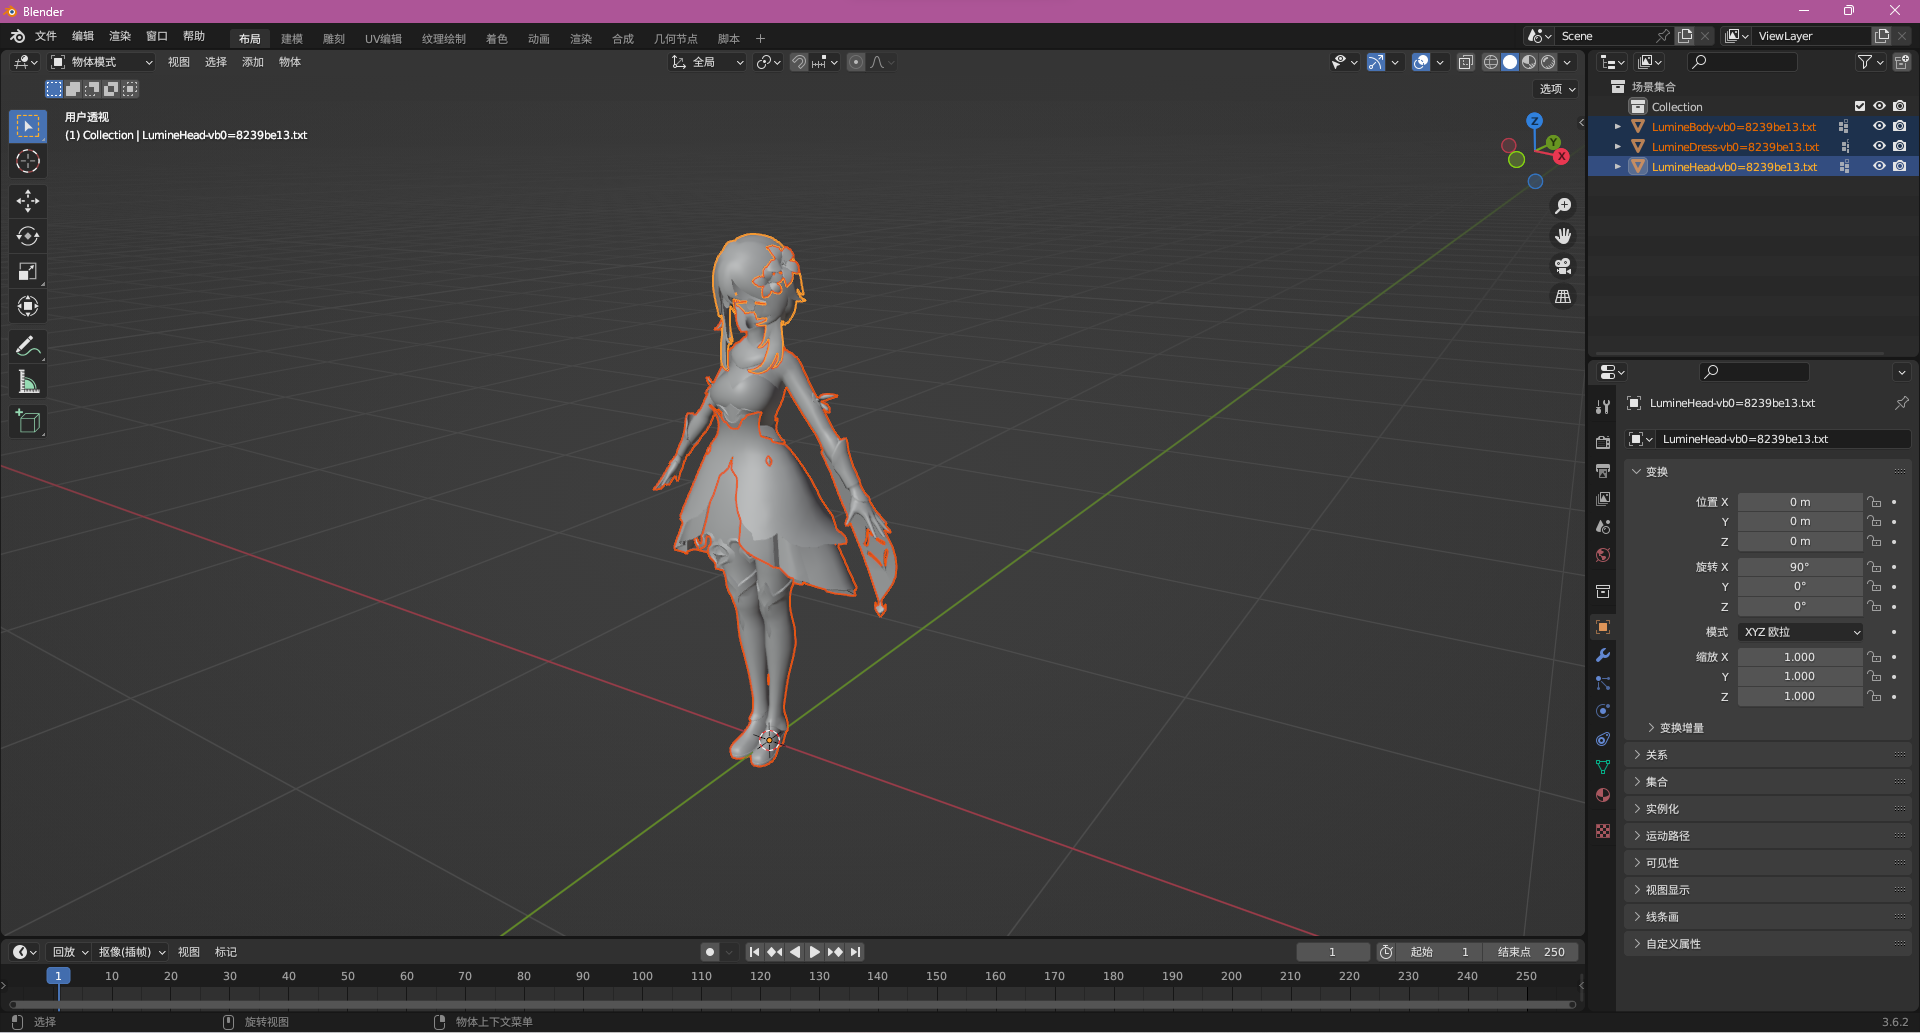
\includegraphics[scale=.15]{2.3Exp1.png}
                    \caption{导入示例}
                \end{figure}
            \par 接下来我们直接导出 MOD, 在顶栏选择 \menu[-]{文件-导出-Export Genshin Mod Folder}, 定位到 \texttt{Lumine} 目录, 确认导出. 此时, 3DM 根目录将会出现一个名为 \texttt{LumineMod} 的文件夹, 这个文件夹就是我们的 MOD 了, 不过这份 MOD 并没有 modify 任何东西. 
            \par 在这个目录中, 我们用 PhotoShop 打开荧妹的纹理贴图, 由于我们要修改的是瞳孔, 因此是 \texttt{Head}, 而修改的内容是其基础色, 因此是 \texttt{Diffuse}, 因此应当打开 \texttt{LumineHeadDiffuse.dds} 文件. 在打开时, 如果图片存在透明度, PhotoShop 会询问是否加载透明度为 Alpha 通道, 遇到时须勾选. 完成你所需要的修改 (你已经学习了所需的 PS 操作, 对吧?), 得到像这样的图片:
                \begin{figure}[H]
                    \centering
                    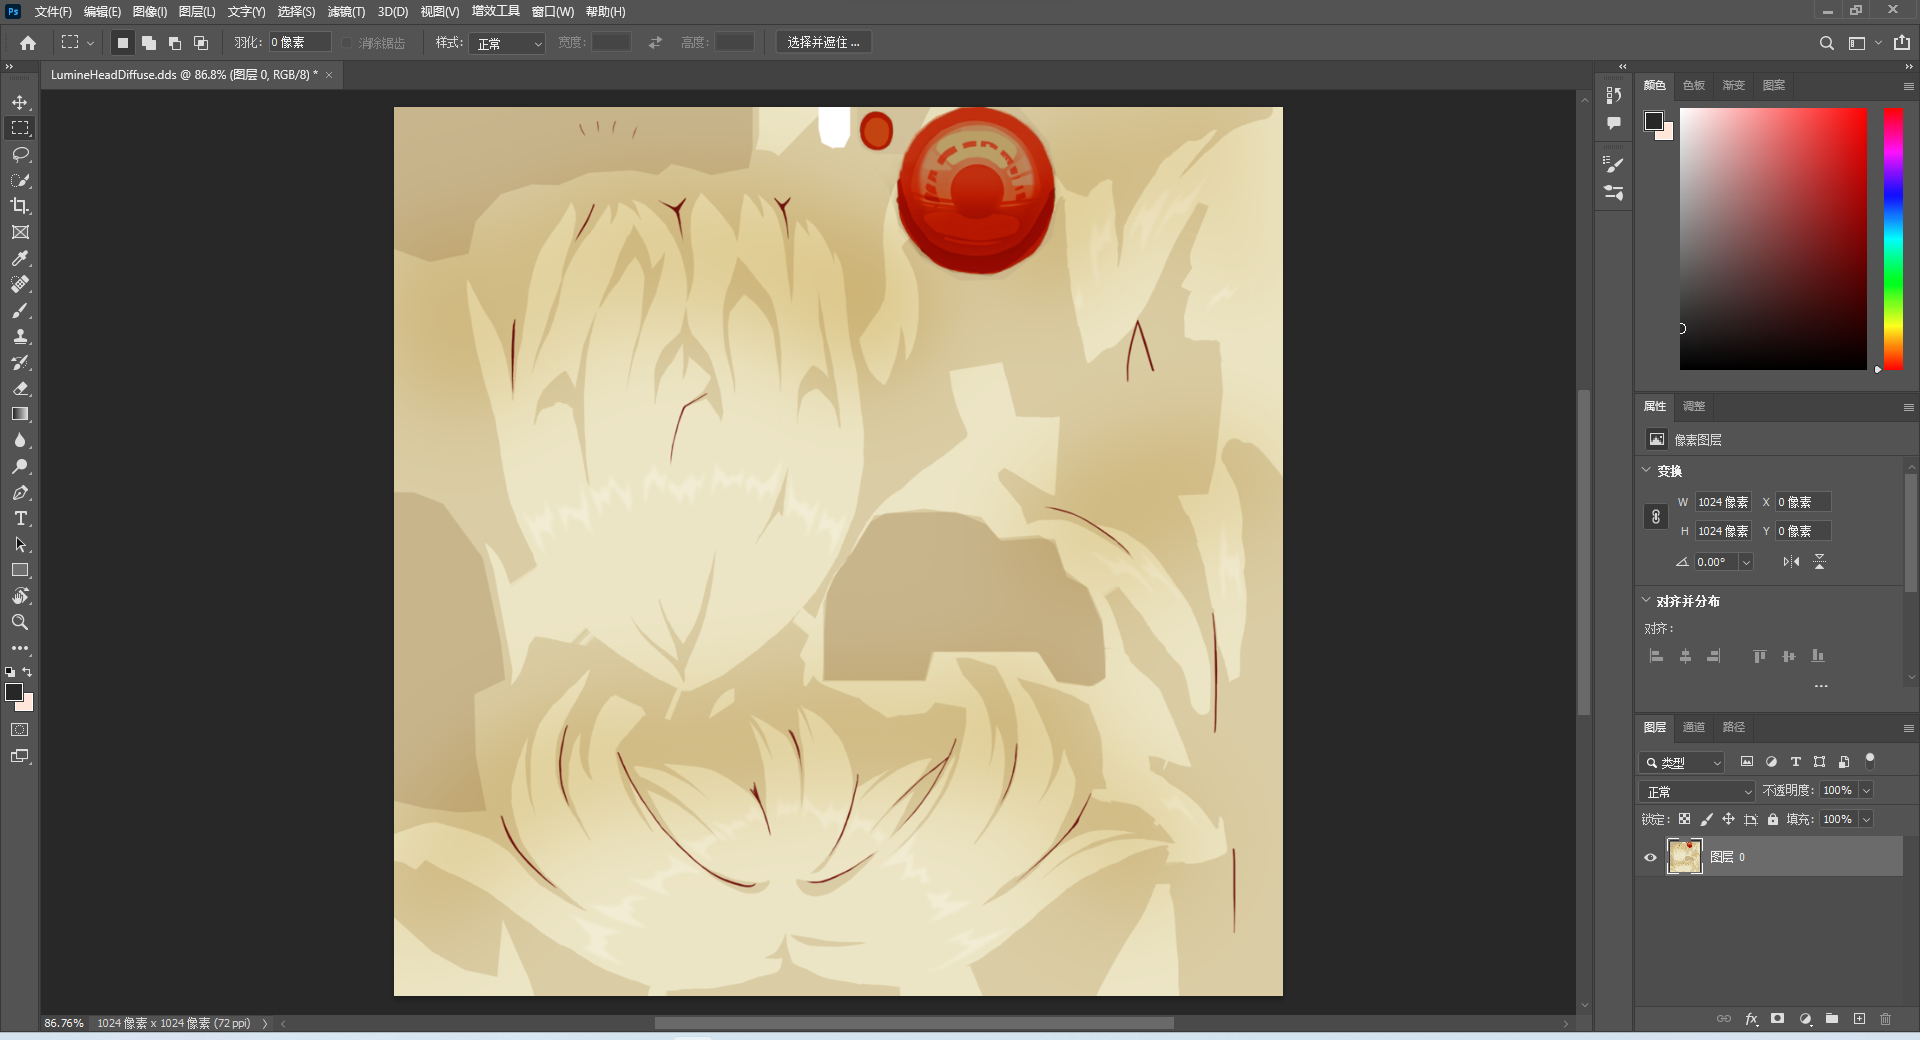
\includegraphics[scale=.15]{2.3Exp2.png}
                    \caption{修改示例}
                \end{figure}
            \par 接下来, 确保工程仅有一个图层, 且没有图层或通道被锁定, 然后存储为 \texttt{.tga} 文件, 再通过 Paint.NET 打开该文件, 存储为 \texttt{.dds} 文件到 \texttt{LumineMod} 目录, 存储选项为 \textbf{BC7 (sRGB, DX11+)}.
            \par 这样, 我们的第一个 MOD 就做好了. 拷贝 MOD 目录至 \texttt{Mods} 目录下, 然后在游戏中按下 \keys{F10} 以重载 MOD, 如果发现荧妹的瞳孔变红, 就说明 MOD 制作、导入成功.
            
        \subsection{没有裙摆的娜维娅——学习删除部件}
            \par 本节操作需要获取娜维娅的源模型.
            \par 在 Blender 中导入娜维娅的源模型, 容易看到娜维娅的模型由 Head, Body, Dress 三个组件构成. 其中 Dress 组件内容为她的裙摆和衣摆, 隐藏组件发现并无多少违和感, 这代表我们可以很方便地做一个去掉 Dress 组件的 MOD.
            \par 如何删除呢? 如果读者尝试直接在物体模式删掉 \texttt{NaviaDress-vb0=f4e09bd7.txt} 这个组件, 又或者聪明些, 进入编辑模式删除该组件所有顶点, 会发现导出 MOD 会导致报错, 这是因为每个组件都必须存在且至少拥有一个面. 正确的做法是仅保留组件的任意一个面并通过缩放和移动藏在模型体内, 再进行导出.
            \par 另外说明, 在编辑模式往往会发现一些并不控制任何边/面的理应属于其他组件的顶点, 这是正常的, 可以放心直接清除, 方式是全选顶点后依次点击 \menu[+]{顶栏第二行+网格+清理+删除松散元素}, 然后在左下角的「删除松散元素」窗口勾选点和边而\textbf{不勾选}面, 回车确认即可清理.
            \par 我们应当已经做出了一个新的 MOD, 但现在有下一个问题: 娜维娅的大腿两侧存在浮空的零件, 选中这些零件会发现这些部分属于 Head 组件, 而该组件包含了手部、颈部、部分身体, 显然不能直接删除. 实际上, 在编辑模式直观地删除多余组件即可, 与前文所述同理, 不会导致任何问题.

        \subsection{让荧妹的发饰换个位置——学习权重传递}
            \par 开宗明义: 权重是 MOD 制作中最恶心的东西(瘫).
            \par 这里推荐 Blender 非官方插件 Handy Weight Edit, 这是一个允许在编辑模式查看模型权重的方便插件. 由于该插件官方版本需付费, 此处不提供下载直链, 请自行查找.
            \par 在 Blender 中, 荧妹头顶的因提瓦特花发饰是这样的:
                \begin{figure}[H]
                    \centering
                    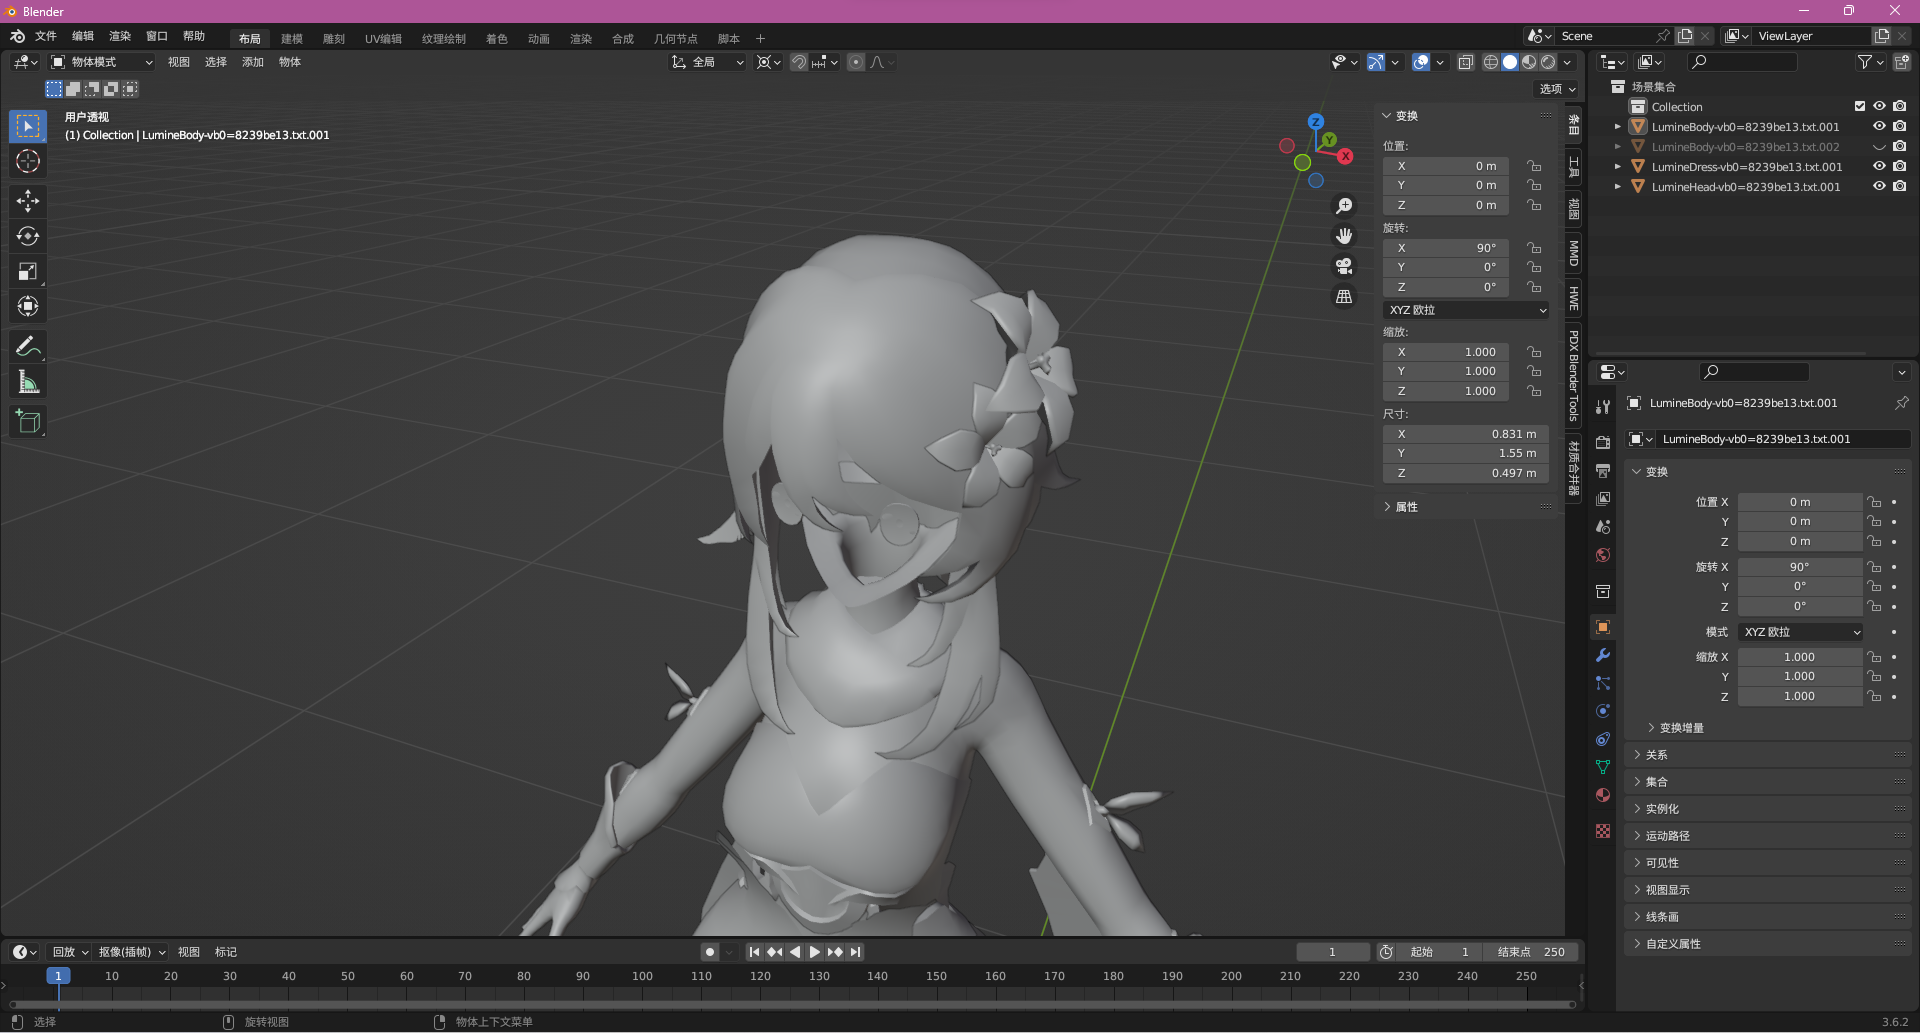
\includegraphics[scale=.15]{2.5Exp1.png}
                \end{figure}
            我们现在的目的是将发饰拖到这里:
                \begin{figure}[H]
                    \centering
                    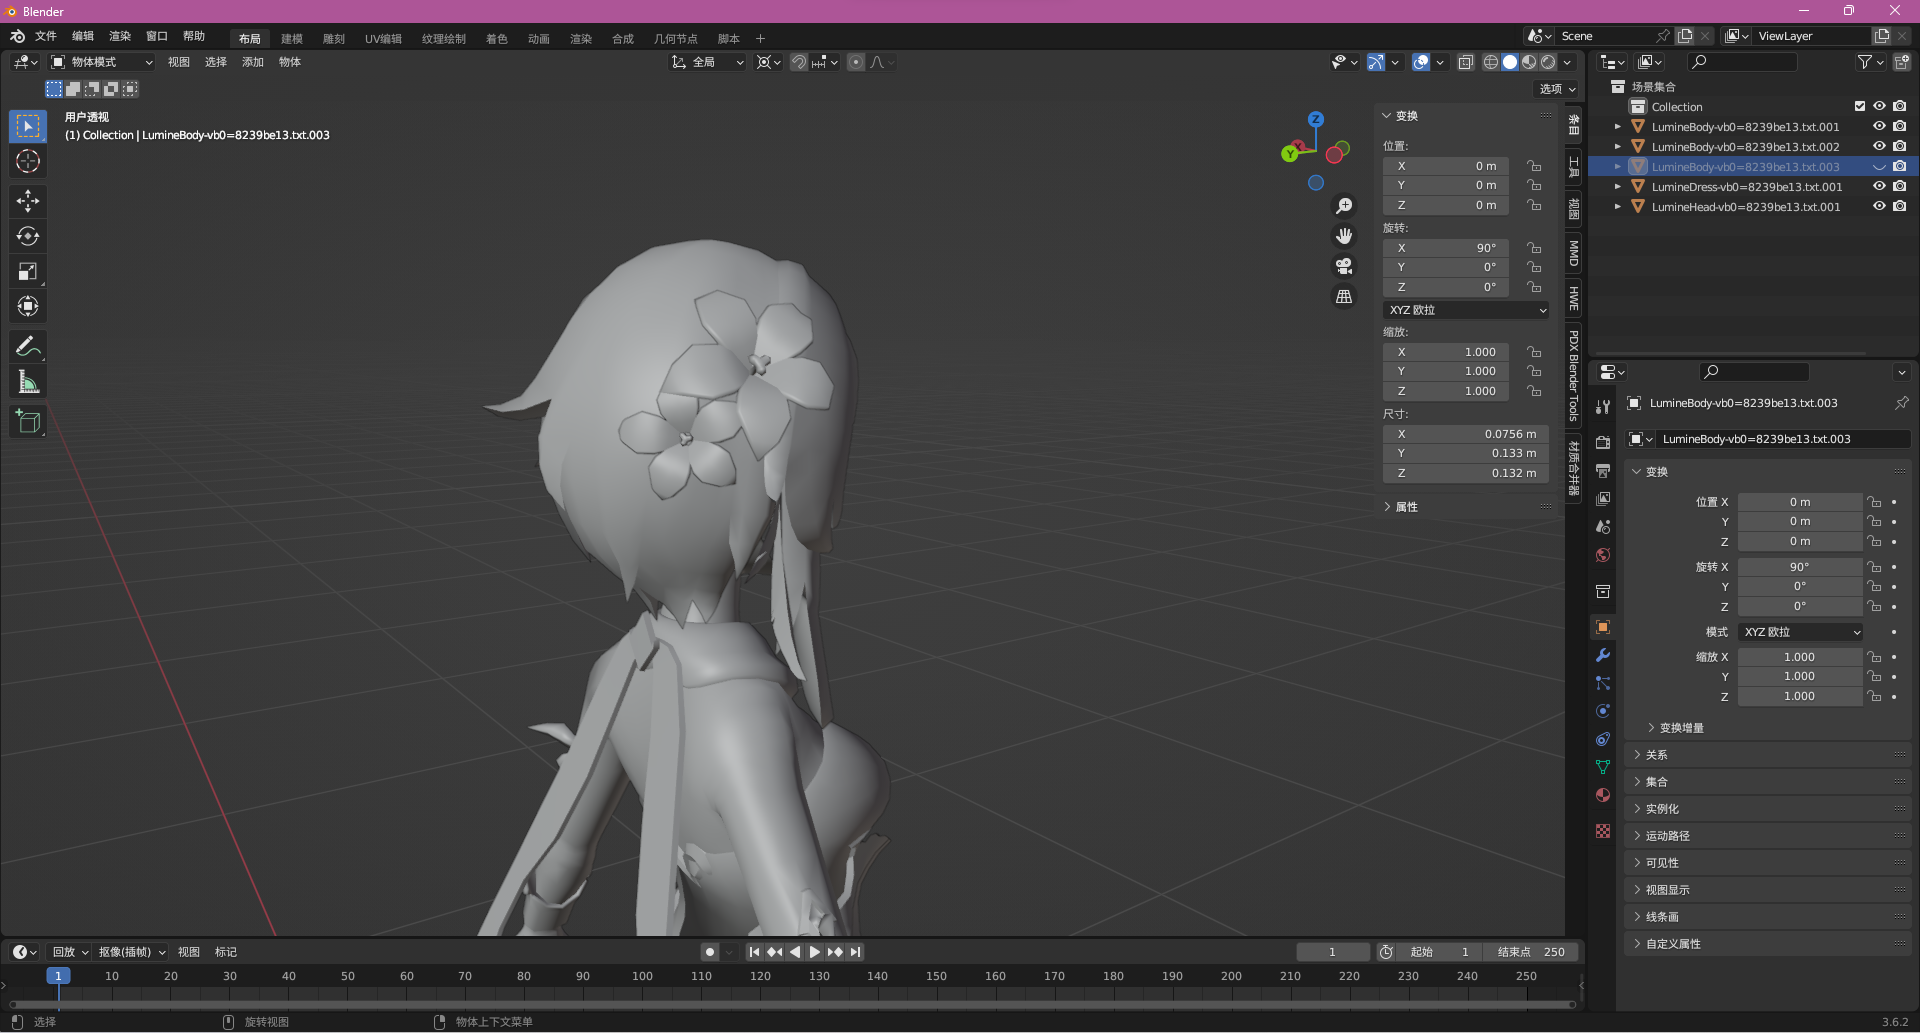
\includegraphics[scale=.15]{2.5Exp2.png}
                \end{figure}
            并保证导出的 MOD 正确渲染.
            \par 相信读到这里的朋友对挪动模型这点小事不在话下, 不过需要注意: 可以先选中分离, 一切编辑完成之后再合并, 但是移动/缩放/旋转一定要在编辑模式下进行, 不要在物体模式下进行, 否则将改变物体的坐标/缩放/旋转, 而非顶点的坐标/相对位置/法线, 而 MOD 需要的是顶点.
            \par 在成功移动到正确位置后, 需要调整已经修改的组件的权重. 为什么要调整权重呢? 实际上, 3DMigoto 会按名称将模型的顶点组绑定至游戏已经提供的骨骼上, 并按顶点组的权重值赋予其被对应骨骼对应的权重. 而这种方式\textbf{无法作用于}使用形态键控制形变的模型上, 这也是为什么基于 3DM 的 MOD 无法修改面部模型. 我们选中模型进入权重编辑模式\footnote{一个更便捷的方式, 但依赖 Handy Weight Edit 插件: 选中对象进入编辑模式, 然后在侧栏打开 \menu{HWE} 以打开插件菜单, 并选择 \menu{Vertex Weight Toggle} 以直接在编辑模式查看对象对应顶点组的权重分布, 然后回到侧栏的 \menu{条目}, 任意选中一个顶点, 此时在条目菜单会显示该顶点归属的所有顶点组, 点击顶点组名称即可切换权重着色.}, 会发现发饰的所有顶点完全属于顶点组 4:
                \begin{figure}[H]
                    \centering
                    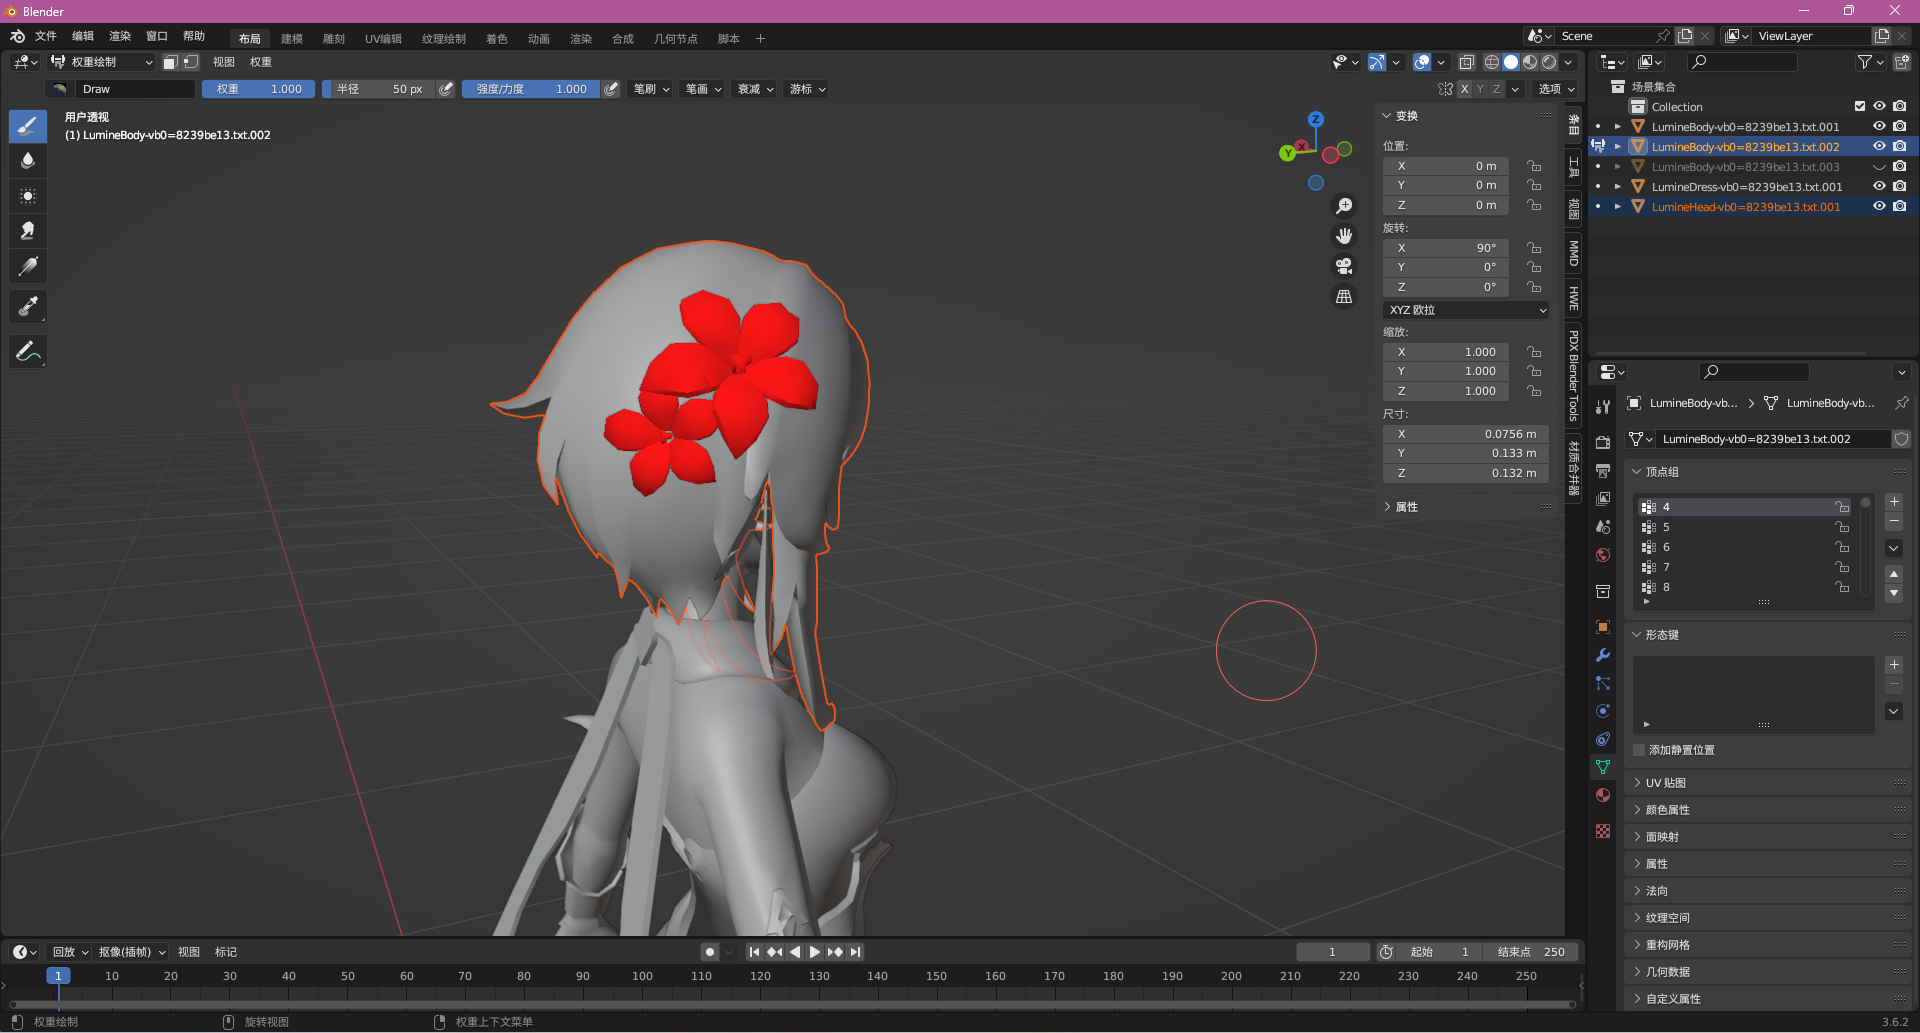
\includegraphics[scale=.15]{2.5Exp3.png}
                \end{figure}
            而再去检查 Head 组件, 会发现顶点组 4 其实就是头部主骨骼. 换言之, 头饰完全由头部主骨骼控制. 其实这意味着我们无需做出多余修改, 直接完成其余琐碎流程即可得到正确运作的 MOD. 但我们这里可以没苦硬吃一下, 来看看头发的顶点组:
                \begin{figure}[H]
                    \centering
                    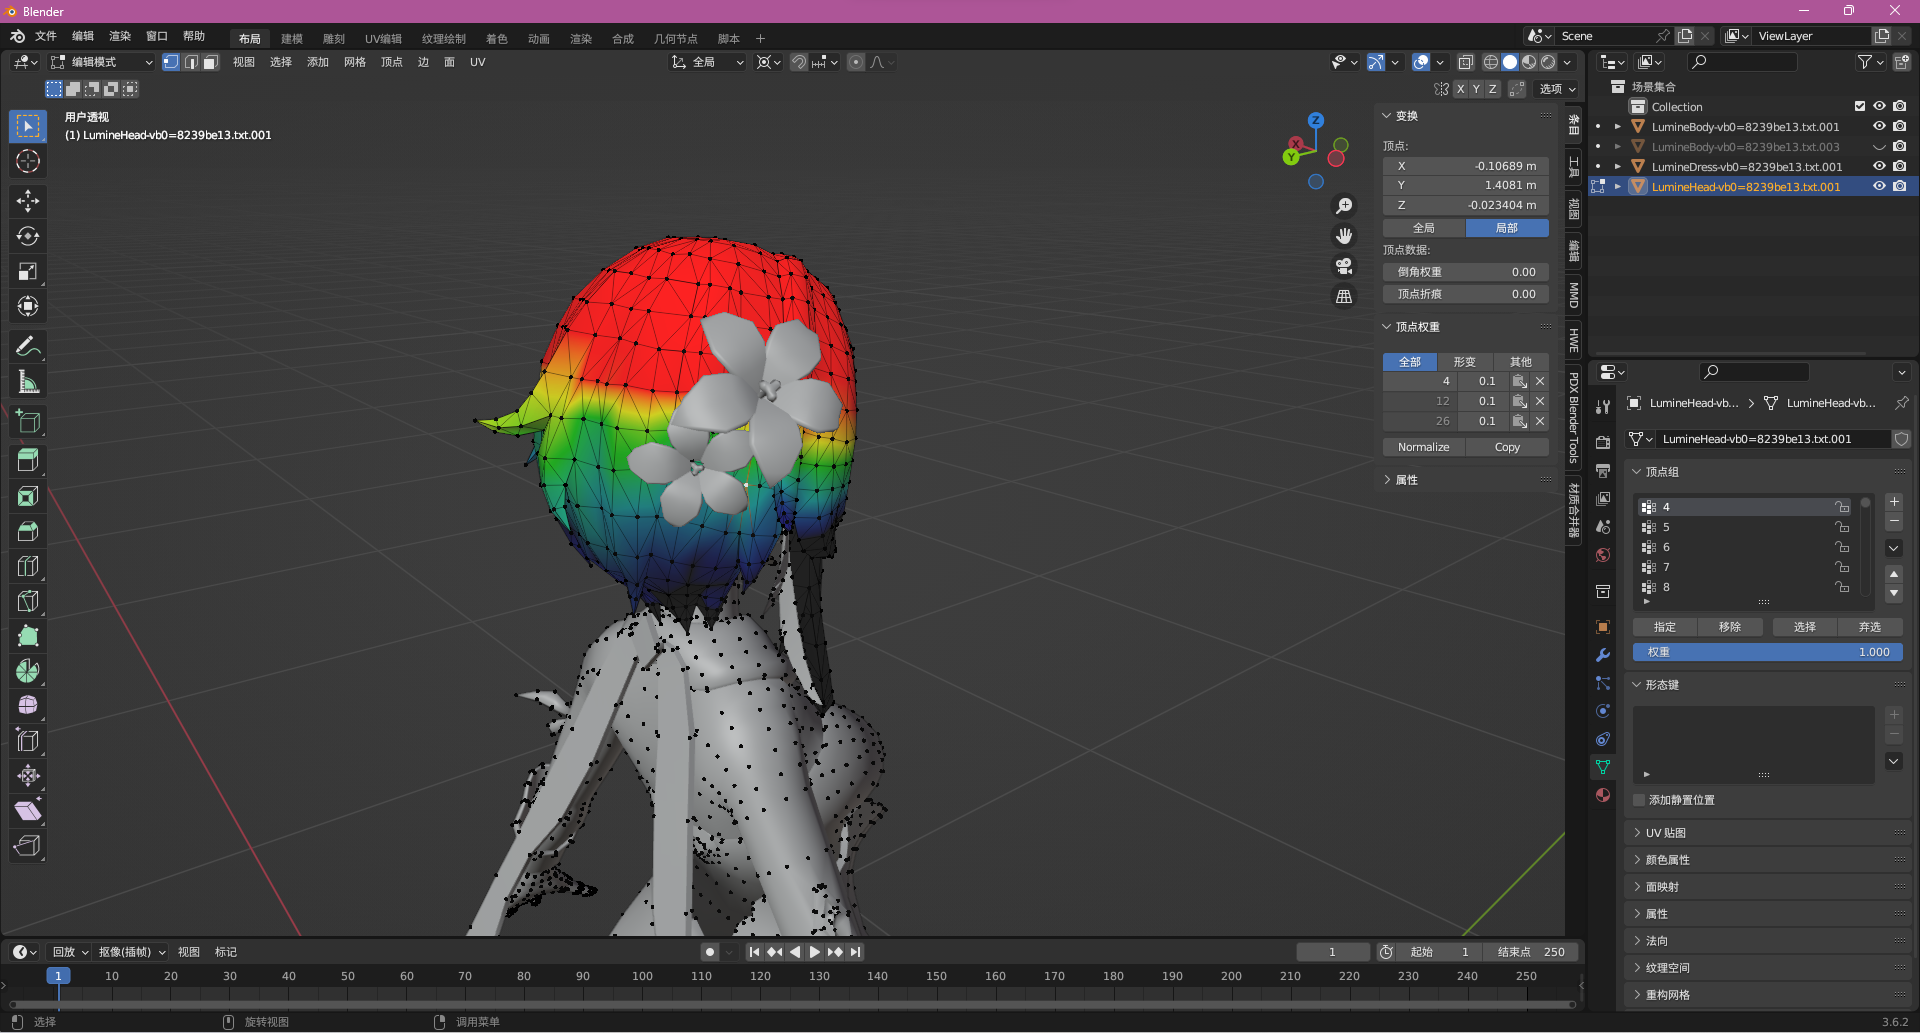
\includegraphics[scale=.15]{2.5Exp4.png}
                \end{figure}
            哎, 我们发现组件所在的新位置对应的头发, 其实并不完全由头部主骨骼控制, 而是部分地被独立的头发骨骼控制. 现在希望让发饰也自然地附着于头发, 一个最方便的做法是权重传递.
            \par 首先请将发饰分离出 Head 组件, 因为权重传递将会作用于组件的所有顶点. 首先选中发饰组件, 进入编辑模式, 全选顶点后在顶栏选择 \menu[+]{顶点+顶点组+从所有组中移除}, 从而删掉该组件所有顶点, 以免无关的顶点组干扰. 请在\textbf{物体模式}下选中头发组件, 然后按住 \keys{Shift} 并选中发饰组件, 接下来进入权重编辑模式, 在顶栏选择 \menu[+]{权重+传递权重}, 再在左下角的细节调整窗口中, \texttt{反勾选}「冻结操作项」, 设定「选择来源层」为「按名称」, 「匹配的目标层」为「全部层」, 其余参数依需求自定, 然后按 \keys{Enter} 确认. 可以检查一下发饰现在的权重, 会发现差不多和头部对应位置的权重相匹配了. 接下来可以直接合并导出, 也可以继续调整细节\footnote{仅对原神而言. 至少在星铁中必须进行之后的操作.}. 在权重编辑模式选择 \menu[+]{权重+光滑}, 然后在调整窗口将子集设为「All Group/全部组」, 根据需要调整迭代次数, 通常不建议超过 3 次. 然后选择 \menu[+]{权重+全部规格化} 并\textbf{反勾选}「锁定活动项」.
            \par 传递权重在不少时候并不能完美解决权重问题, 如果需要, 建议反复调整, 包括手动绘制权重等麻烦至极的操作.
        \subsection{让荧妹戴上娜维娅的礼帽——学习 UV 与纹理编辑}
            \par 将礼帽复制粘贴过来.——然后得到一坨古神.
            \par 聪明些, 粘贴过来后, 做好权重.——然后得到一顶古神配色的礼帽.
            \par 实际上, 对于不属于原组件的面组, 其自带的 UV 与所提供的纹理往往并不匹配. 在 UV 编辑窗口查看以 \texttt{.png} 格式转储\footnote{通过 Paint.NET 完成, 有时有必要 \keys{Ctrl+Alt+I} 以反转图片透明度, 从而使大部分纹理在 \texttt{.png} 中可见.}的  \texttt{LumineBodyDiffuse} (如果你希望将礼帽合并至 Body), 会发现礼帽的 UV 网格和纹理完全不匹配, 我们需要做一个新的 Diffuse 纹理以容纳原来两份不同的纹理.
            \par 通常的做法是拓展其中一个纹理图片的画布大小, 将另一个纹理粘贴进去:
            \begin{figure}[H]
                \centering
                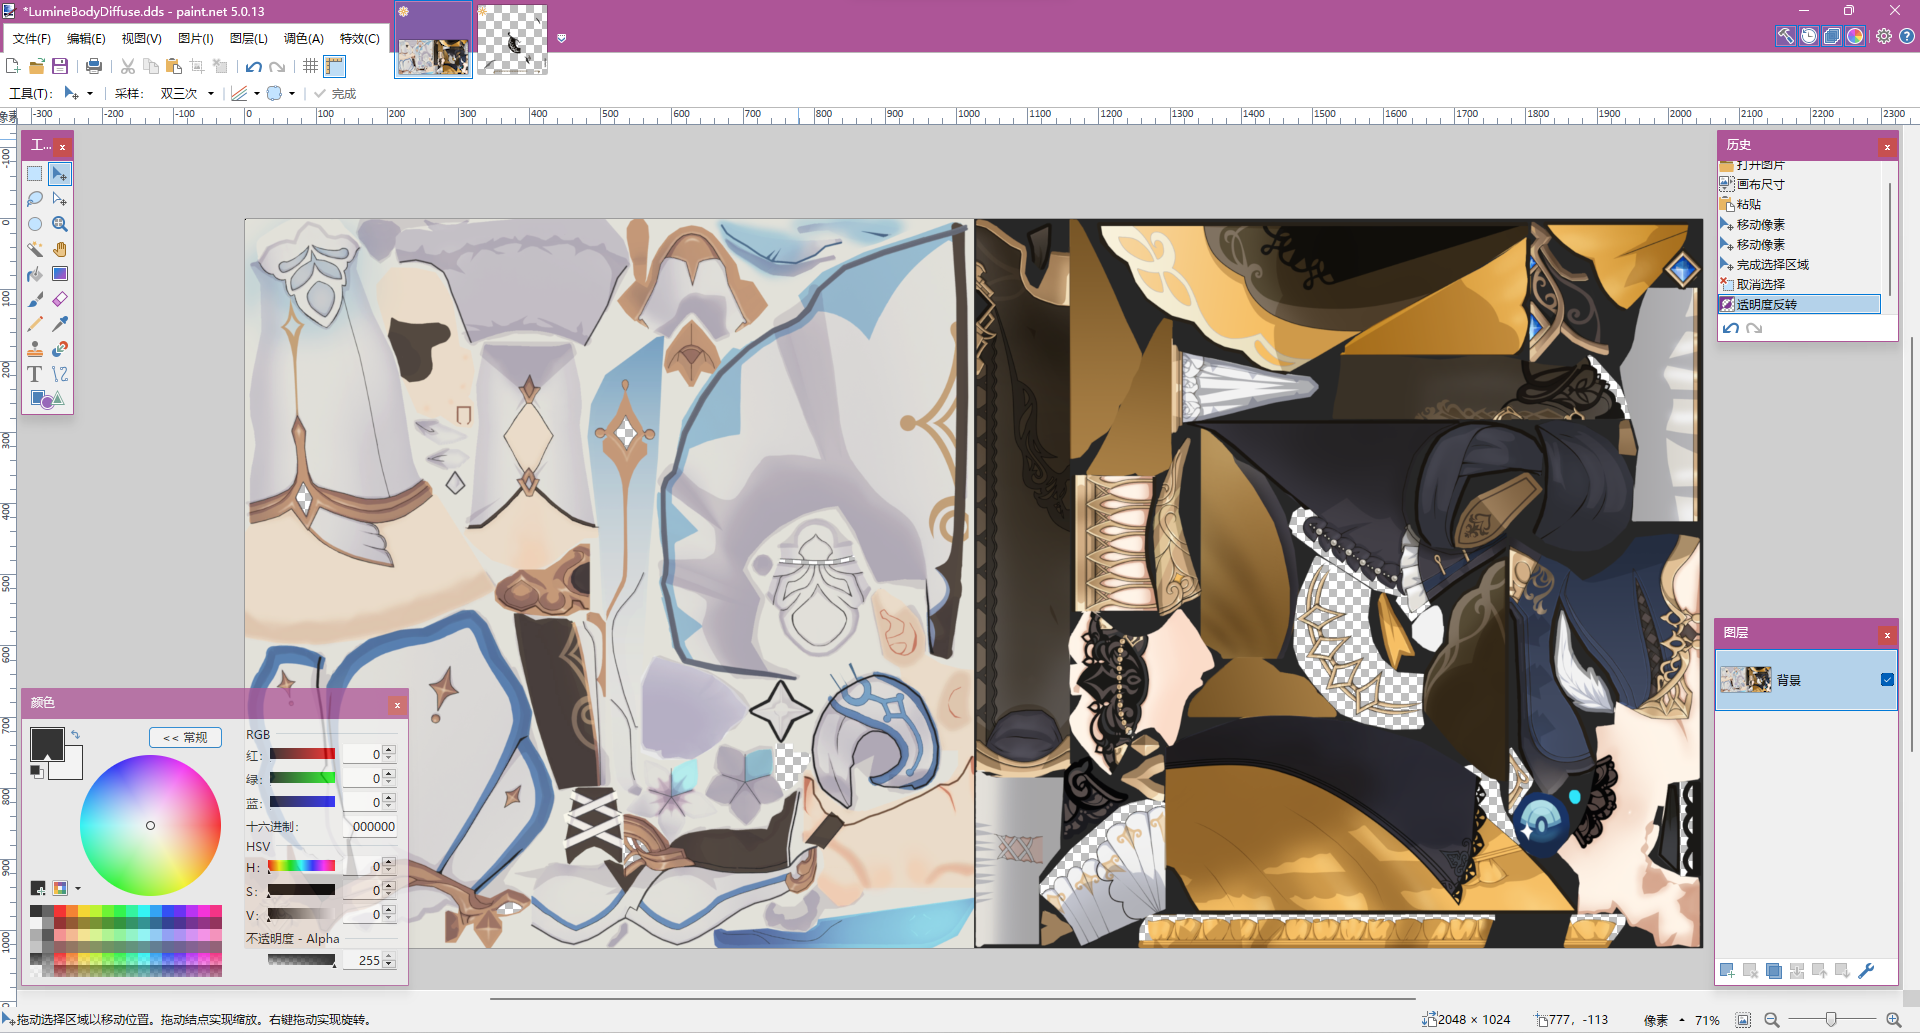
\includegraphics[scale=.15]{2.6Exp1.png}
            \end{figure}
            \par 需要指出上图在导出时需要自行调整透明度, 对于荧妹来说, 透明度为 100\% 的像素点将会如实渲染, 而娜维娅的纹理中, 透明度有其他用途, 如果自己的 MOD 希望更加细致, 应当消除娜维娅纹理中自带的透明度.
            \par 接下来调整模型 UV 以使 UV 网格正确匹配新的纹理. 这里说明 UV 的一个工作机制, 阅读有困难的读者酌情略过:
            \begin{quotation}
                {\color{gray}所谓 UV, 当理解为二维坐标系 \(O\dash uv\), 区别于顶点自身所在的坐标系 \(O\dash xyz\), 应当理解顶点作为 \(O\dash xyz\) 之子集 \(V=\{v_1,v_2,\dots,v_n\colon\forall i, v_i\in O\dash xyz\}\), 而 UV 网格的本质是一个映射 \(\varphi\colon V\to O\dash uv, v\mapsto p\), 将三维的顶点映射到二维的网格点, \textbf{并保持边关系和面关系}, 网格点内部存储的坐标数据 \((u,v)\) 通常限制在闭区间 \([0,1;0,1]\) 内, 坐标 \((0,0)\) 对应左下角, \((1,1)\) 对应右上角.}
            \end{quotation}
            换言之, 无论给出的纹理文件之纵横比如何变换, 尺寸如何变换, 其整个图像都被等效为了区间 \([0,1;0,1]\), 而将整张 UV 网格拉伸铺满整个图像. 在比较少见的情况中, 部分网格点会出现在图像外侧, 也就是说其坐标脱离了 \([0,1;0,1]\) 之限制, 此时可以理解为, 纹理图像实际上循环平铺了整个 \(O\dash uv\) 平面, 只不过通常仅需要用到其 \([0,1;0,1]\) 之内的部分, 也仅看得到这部分. 更本质地说, 网格的 \(uv\) 坐标实际上在 \(\Mod_{\mathbb{R}^2} (1,1)\) 同余意义下等价.
            \par 对于一个三点确定的三角面, 其将读取三点各自对应的 UV 网格点, 并截取三网格点围成的三角区域, 截取这部分纹理, 绘制到三维模型对应的面上去. 对于非三角的面, 包括四边面和多边面, 工作细节会更复杂一些, 不过整体流程一致.
            \par 选择礼帽对象, 进入编辑模式全选顶点后打开 UV 编辑器, 导入我们制作好的纹理图像的 \texttt{.png} 版本,可以看到预期中占据右半边的网格实际被拉伸占据了整个图像. 需要做的工作非常明了: 横向缩放整个 UV 网格至 0.5 倍, 并横向移动整个 UV 网格以使其贴合纹理. UV 编辑器内的操作与快捷键基本和 3D 视图内一致, 按照直觉完成即可.
            \par 接下来选择荧妹 Body 对象, 进行相近的操作. 这是因为我们要将两份无关的 UV 塞到一起, 而原 UV 势必要腾出位置来——也就是按照我们纹理图像中的左半边区域进行缩放移动. 总之, 应当将 UV 网格调整至下图所示:
            \begin{figure}[H]
                \centering
                \subfigure{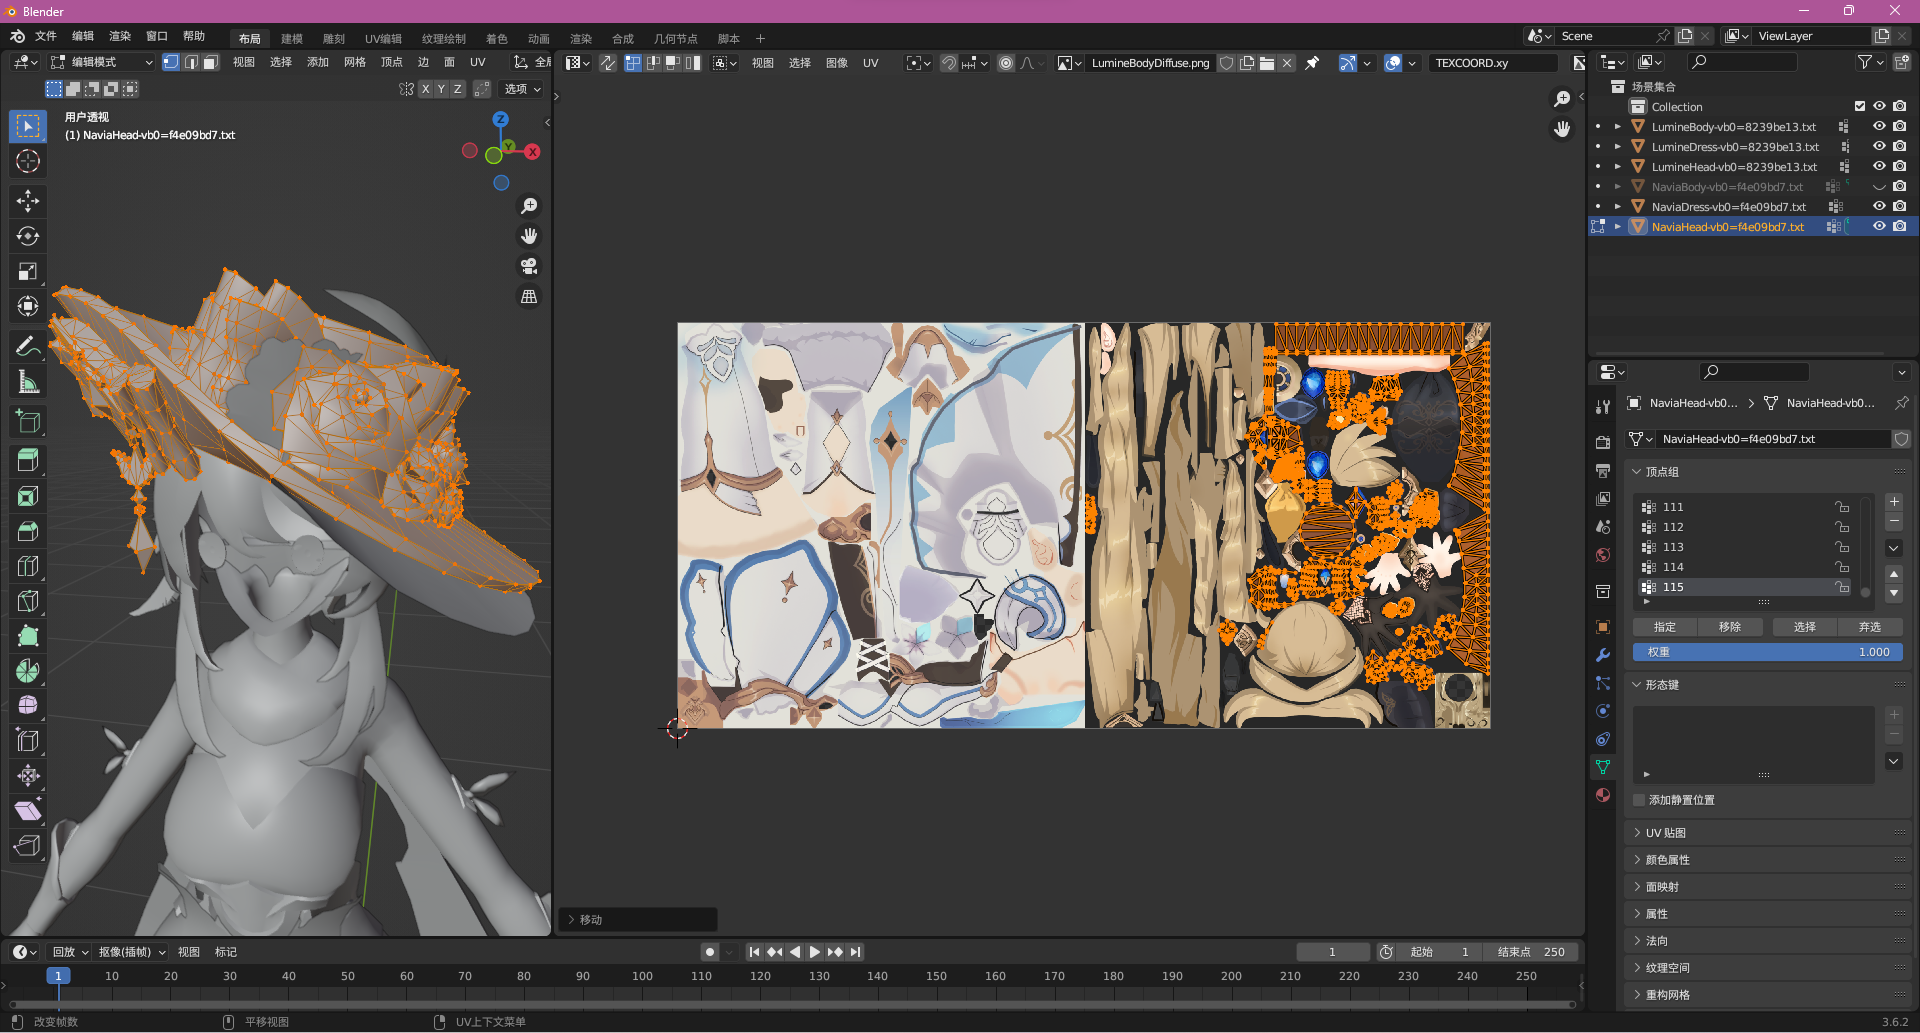
\includegraphics[scale=.12]{2.6Exp2.1.png}}
                \subfigure{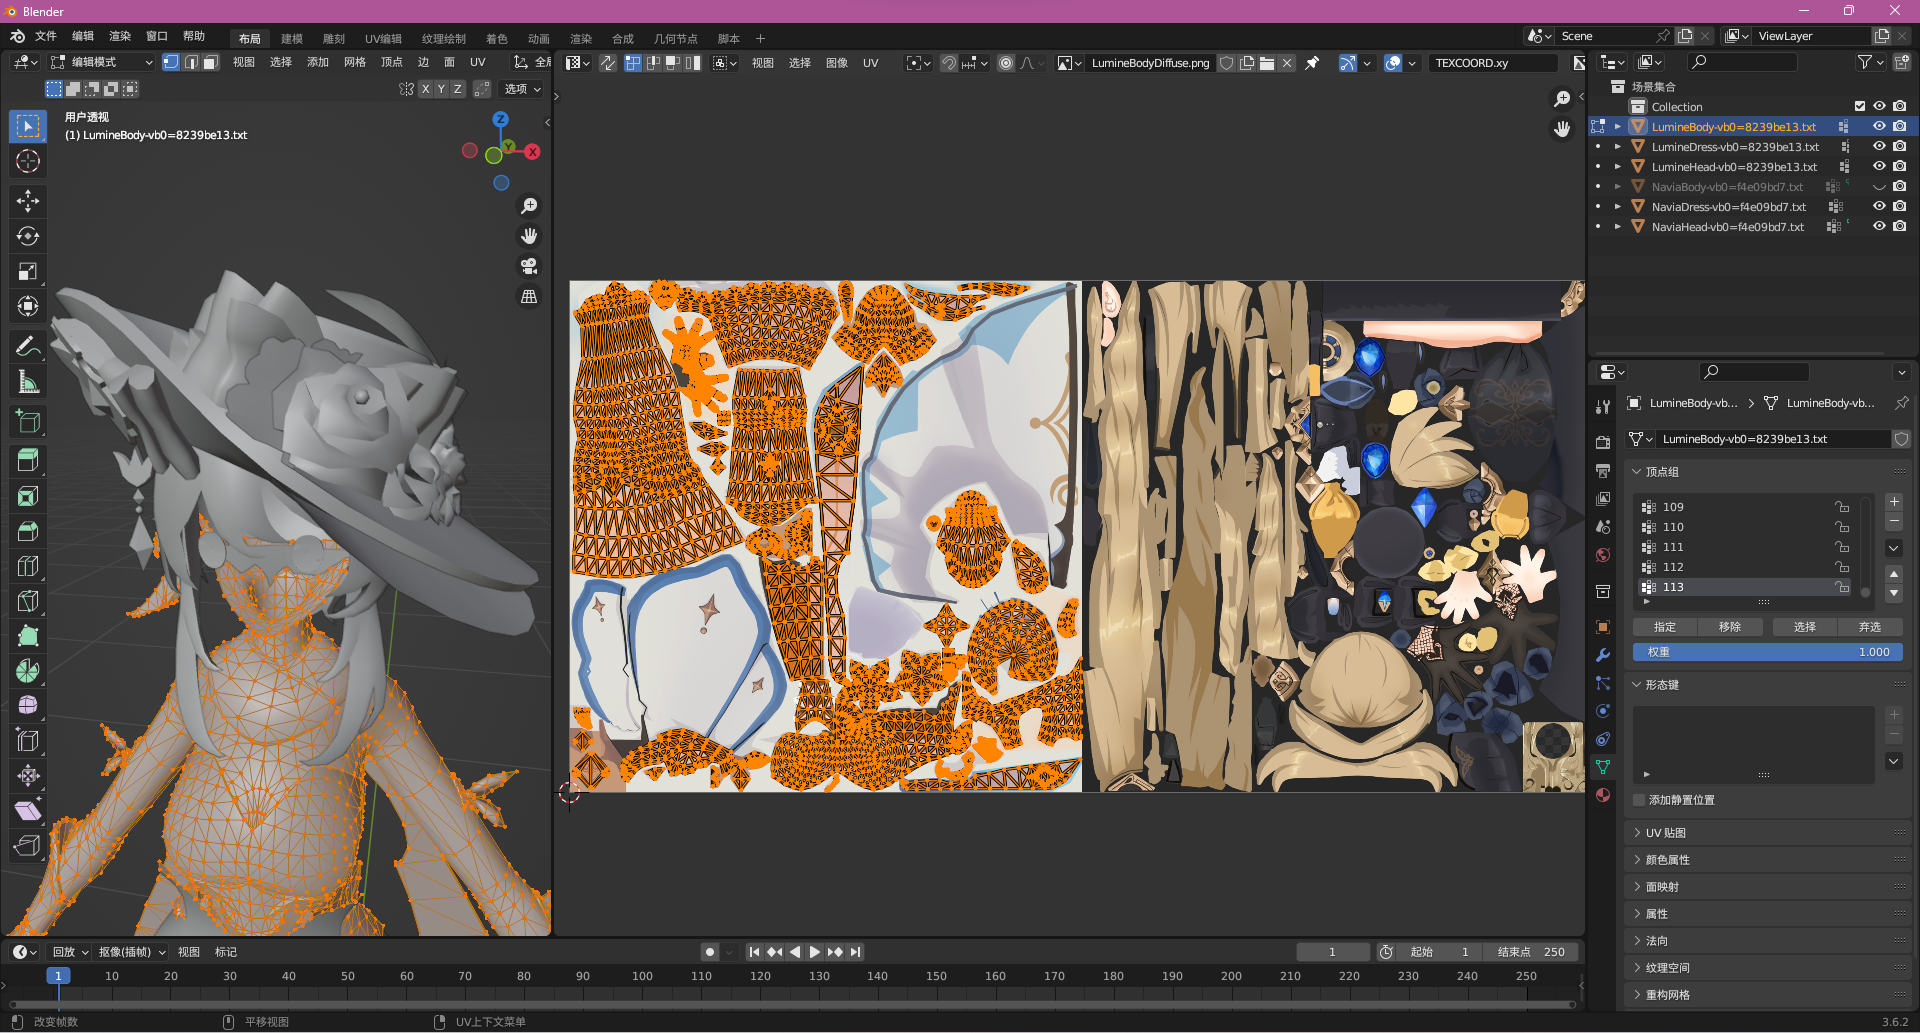
\includegraphics[scale=.12]{2.6Exp2.2.png}}
            \end{figure}
            然后根据上一节所述, 调整权重. 这里推荐将整个礼帽完全归于头部骨骼.
            \par 权重调整完成后, 将礼帽合并\texttt{至}荧妹的 Body 对象上, 即可导出 MOD 了.
            \par 但读者此时还不能得到正常渲染的 MOD, 大致的配色没有问题, 但会有奇怪的明显色差, 这是因为我们修改了 Diffuse Map, 而尚未修改 Light Map 和 Normal Map.
            \par Light Map, 即光照映射. 一个面的着色, 除了基本的漫反射纹理 Diffuse Map 之外, 还应当处理其光照反射性质, 有多粗糙? 有多能反光? 环境光遮蔽程度如何? 这些都需要在 Light Map 中控制.
\iffalse
            {\par 具体来说, 一个以 RGBA 方式着色图片可以等效为四个等尺寸灰度图片的叠加, 称作该图片的四个\textbf{通道}, 分别是红通道 (\textbf{R}ed), 绿通道 (\textbf{G}reen), 蓝通道 (\textbf{B}lue), 透明通道 (\textbf{A}lpha). 从而, RGBA 图片的每个像素点可被视作一个四维向量 \((R,G,B,A)\), 而该向量取值于 \((\mathbb{Z}\cap[0,255])^4\), 换言之, 每个分量均为 0 到 255 之间的某个整数.
            \par 显然, 这多出来的一份 Light Map 贴图并不用于直接着色, 但其内部数值的格式很方便于分通道调控每个像素点的光照性质. 以原神 MOD 为例, 其 R, G, B, A 四个通道分别控制: 
                \begin{description}
                    \item[Red] 用于控制该点的金属度, 使金属度贴图 MetalMap 生效. 0 代表完全不是金属, 255 代表完全是金属.
                    \item[Green] 用于控制环境光遮蔽 (\textbf{A}mbient \textbf{O}cclusion) 强度. 这将控制该点接受环境光的程度. 在一般的渲染中, 环境光遮蔽由一定计算决定, 使拐角处的顶点接受更少的环境光. 但是在游戏渲染中, 这样的计算通常难以完成, 因为性能需求过高而无法实时计算. 此时, AO 通道将方便地直接指定静态的 AO 值. 通常, 0 表示永远不被光照, 128 表示永远接受光照 (神之眼), 在原神中, 全部设定为 128 (即 50\%) 即可得到正常光照.
                    \item[Blue] 用于控制高亮反光. 字面意思, 控制镜面反射的强度. 高亮反光需要金属度辅助, 对纯粹的非金属 ($R=0$) 来说, B 通道几乎不影响着色, 而随着金属度的增加, 高亮反光将会越来越集中, 最后将会变成完全的镜面反射. B 的值控制镜面反射本身的强度.
                    \item[Alpha] (本段还得改) 控制光泽强度. 
                \end{description}
}
\fi
            \par 
            \par 本节内容稍微偏多, 因为着色本身确实是一个很大的流程. 
        \subsection{扒掉荧妹的衣服!——学习逆向 MOD}
        \subsection{荧妹! 大欧派!——学习简单的雕刻}
        \subsection{自定义玩家头像——学习 2D 纹理 MOD 的制作}
        \subsection{让荧妹变成符太卜!——不同游戏之间的模型移植}

    \section{Engineer}
        Only self-using notes.
        \subsection{Linear Algebra Basic}
            \par Reviewing about some basic linear algebra.
            \begin{definition}
                An \(n\)--tuple \((x_1, x_2, \dots, x_n)\) denotes recursively \(((x_1, \dots, x_{n-1}), x_n)\), and a 2-tuple \((x,y)\) denotes set \(\{x, \{x,y\}\}\)\ (by Kuratowski).
            \end{definition}
            A vector can not be a tuple, and a tuple can not be a vector.
            \begin{definition}
                A \textbf{Vector Space} denotes a 4--tuple \((\mathbb{F}, V; \mathbf{0}_V; +_V, \cdot)\) that:
                    \begin{itemize}
                        \item \(\mathbb{F}\) is a field \((F; 0_F, 1_F; +_F, \cdot_F)\);
                        \item \(V\) is one non-empty set;
                        \item \(+_V\) is an operator on \(V\) that \((V; \mathbf{1}_V; +_V)\) is an Abelian group;
                        \item \(\cdot\) is an operator between \(\mathbb F\) and \(V\) that:
                            \begin{itemize}
                                \item \(\forall a\in\mathbb{F},\forall v\in V, av\in V\);
                                \item \(\forall v\in V, 1_Fv=v\);
                                \item \(\forall a\in\mathbb{F},\forall v,w\in V, a(v+_Vw)=av+_Vaw\);
                                \item \(\forall a,b\in\mathbb{F},\forall v\in V, (a+_Fb)v=av+_Fbv\).
                            \end{itemize}
                    \end{itemize}
            \end{definition}
        \subsection{Transformation}
        \subsection{Rasterization}
        \subsection{Shader}
        \subsection{Buffer}
        
\end{document}